\documentclass{article}
\usepackage{geometry}
\usepackage{paralist}
\usepackage[T1]{fontenc}
\usepackage{reledmac}
\usepackage{changepage}
\usepackage{amsmath}
\usepackage{scalerel,amssymb}

\graphicspath{{./snippets/}}

\usepackage{fancyhdr}
\fancyhead[L]{
	\begin{tabular}{l}
		\LARGE \textbf{\textsc{Concurrency}} \\
		\Large Assignment 01
	\end{tabular}
}
\fancyhead[R]{
	\begin{tabular}{r}
		16-124-836 \\
		Marcel \textsc{Zauder}
	\end{tabular}
}
\renewcommand{\headrulewidth}{0.4pt}
\fancyfoot[C]{\thepage}
\renewcommand{\footrulewidth}{0.4pt}

\usepackage{hyperref}

\begin{document}
	\pagestyle{fancy}
	
	\section*{Question 01: Prime Numbers}
	\begin{adjustwidth}{2em}{2em}
		In the following section, I will recap the results of the \textit{primeFinder}-algorithm. I have used an Intel-Core i5-7200U Quad-Core CPU. I also added the cases of $4^{11}$, $4^{12}$, $4^{13}$, and $4^14$ because the difference at $4^{10}$ between the range and ticketing approach was nearly negligible:
		\subsection*{Case 1: $4^{10}$}
		\begin{adjustwidth}{2em}{2em}
			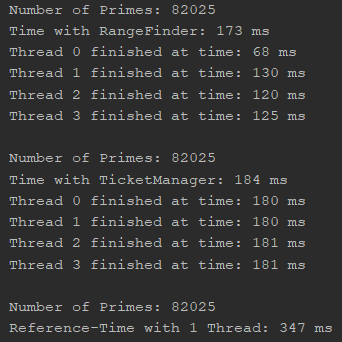
\includegraphics[scale=0.6]{Output_power_10.png}
			\subsubsection*{\textsc{RangeFinder}}
			\begin{adjustwidth}{1em}{}
				The \textsc{RangeFinder}-Threads takes 173ms to finish searching for primes. But from the output we can see that the thread which will finish first, only is computing half of the time and the rest of it he is waiting for the others to finish.
			\end{adjustwidth}
			\subsubsection*{\textsc{Ticketing-System}}
			\begin{adjustwidth}{1em}{}
				The \textsc{Ticketing-System} needs surprisingly longer than the \textsc{RangeFinder}-Threads. The cause for this could be the large overhead which is produced when each thread is fetching (synchronized) their next number to compute, so I added several more cases with more numbers to check this assumption. In contrast to the \textsc{RangeFinder} approach, here all the threads will finish at nearly the same time, so no thread will be idle for too long.
			\end{adjustwidth}
			\subsubsection*{\textsc{One-Thread-Reference + Speedup}}
			\begin{adjustwidth}{1em}{}
				For one thread the computation takes significantly longer, so we compute the speed-up: \\
				\begin{enumerate}[]
					\item \textsc{RangeFinder-SpeedUp}: \\
					$\textit{SpeedUp} \ = \ \frac{\textit{OldExecutionTime}}{\textit{NewExecutionTime}} \ = \ \frac{347}{173} \ = \ 2.006$
					\item \textsc{Ticketing-System-SpeedUp}: \\
					$\textit{SpeedUp} \ = \ \frac{\textit{OldExecutionTime}}{\textit{NewExecutionTime}} \ = \ \frac{347}{184} \ = \ 1.886$
				\end{enumerate}
				\hfill \\
				For both approaches the speedup is approximately 2, which is what we would expect (faster but not 4 times faster because we have synchronized code snippets).
			\end{adjustwidth}
		\end{adjustwidth}
		
		\subsection*{Case 2: $4^{11}$}
		\begin{adjustwidth}{2em}{2em}
			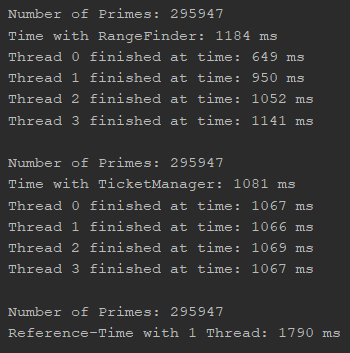
\includegraphics[scale=0.6]{Output_power_11.png}
			\subsubsection*{\textsc{RangeFinder}}
			\begin{adjustwidth}{1em}{}
				The \textsc{RangeFinder}-Threads takes 1184ms to finish searching for primes. The first one to finish needs 649ms for its range part (again approximately half the computing time of the last one).
			\end{adjustwidth}
			\subsubsection*{\textsc{Ticketing-System}}
			\begin{adjustwidth}{1em}{}
				Now the \textsc{Ticketing-System} has overtook the \textsc{RangeFinder} and terminates faster, because every thread is working all the time and there is no idle time
			\end{adjustwidth}
			\subsubsection*{\textsc{One-Thread-Reference + Speedup}}
			\begin{adjustwidth}{1em}{}
				The \textsc{One-Thread-Reference} needs 1790ms, the speedup is therefore: \\
				\begin{enumerate}[]
					\item \textsc{RangeFinder-SpeedUp}: \\
					$\textit{SpeedUp} \ = \ \frac{\textit{OldExecutionTime}}{\textit{NewExecutionTime}} \ = \ \frac{1790}{1184} \ = \ 1.512$
					\item \textsc{Ticketing-System-SpeedUp}: \\
					$\textit{SpeedUp} \ = \ \frac{\textit{OldExecutionTime}}{\textit{NewExecutionTime}} \ = \ \frac{1790}{1081} \ = \ 1.656$
				\end{enumerate}
				\hfill \\
				In this case it is still faster but the speedup is not as huge as before which could be because of the very small time differences in the first case.
			\end{adjustwidth}
		\end{adjustwidth}
		
		\newpage
		
		\subsection*{Case 3: $4^{12}$}
		\begin{adjustwidth}{2em}{2em}
			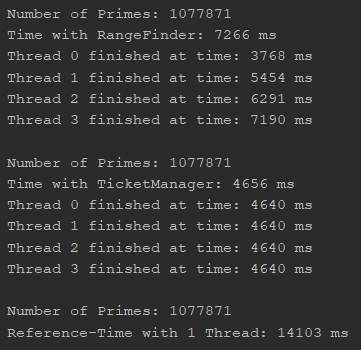
\includegraphics[scale=0.6]{Output_power_12.png}
			\subsubsection*{\textsc{RangeFinder}}
			\begin{adjustwidth}{1em}{}
				The \textsc{RangeFinder}-Threads takes 7266ms to finish searching for primes. The first one to finish needs 3768ms for its range part (again approximately half the computing time of the last one).
			\end{adjustwidth}
			\subsubsection*{\textsc{Ticketing-System}}
			\begin{adjustwidth}{1em}{}
				Now the \textsc{Ticketing-System} is much faster than the \textsc{RangeFinder} with only 4656ms.
			\end{adjustwidth}
			\subsubsection*{\textsc{One-Thread-Reference + Speedup}}
			\begin{adjustwidth}{1em}{}
				The \textsc{One-Thread-Reference} needs 14103ms, the speedup is therefore: \\
				\begin{enumerate}[]
					\item \textsc{RangeFinder-SpeedUp}: \\
					$\textit{SpeedUp} \ = \ \frac{\textit{OldExecutionTime}}{\textit{NewExecutionTime}} \ = \ \frac{14103}{7266} \ = \ 1.941$
					\item \textsc{Ticketing-System-SpeedUp}: \\
					$\textit{SpeedUp} \ = \ \frac{\textit{OldExecutionTime}}{\textit{NewExecutionTime}} \ = \ \frac{14103}{4656} \ = \ 3.029$
				\end{enumerate}
				\hfill \\
				In this case we can see that the \textsc{RangeFinder} is approximately 2 times faster than the sequencial approach. The \textsc{Ticketing-System} is even 3 times faster.
			\end{adjustwidth}
		\end{adjustwidth}

		\newpage		
		
		\subsection*{Case 4: $4^{13}$}
		\begin{adjustwidth}{2em}{2em}
			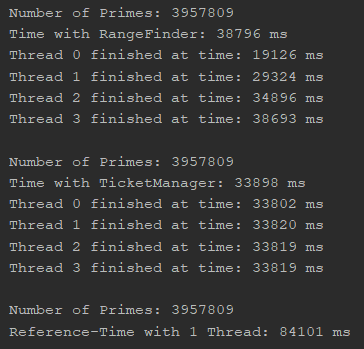
\includegraphics[scale=0.6]{Output_power_13.png}
			\subsubsection*{\textsc{RangeFinder}}
			\begin{adjustwidth}{1em}{}
				The \textsc{RangeFinder}-Threads will take 38796ms to finish searching for primes. The first one to finish needs 19126ms for its range part (again approximately half the computing time of the last one).
			\end{adjustwidth}
			\subsubsection*{\textsc{Ticketing-System}}
			\begin{adjustwidth}{1em}{}
				Now the \textsc{Ticketing-System} is faster than the \textsc{RangeFinder} with only 33898ms but not as much as before. A reason for this could be that with higher numbers there are much less primes so the method isPrime will output false more often and frequently than before.
			\end{adjustwidth}
			\subsubsection*{\textsc{One-Thread-Reference + Speedup}}
			\begin{adjustwidth}{1em}{}
				The \textsc{One-Thread-Reference} needs 84101ms, the speedup is therefore: \\
				\begin{enumerate}[]
					\item \textsc{RangeFinder-SpeedUp}: \\
					$\textit{SpeedUp} \ = \ \frac{\textit{OldExecutionTime}}{\textit{NewExecutionTime}} \ = \ \frac{84101}{38796} \ = \ 2.168$
					\item \textsc{Ticketing-System-SpeedUp}: \\
					$\textit{SpeedUp} \ = \ \frac{\textit{OldExecutionTime}}{\textit{NewExecutionTime}} \ = \ \frac{84101}{33898} \ = \ 2.481$
				\end{enumerate}
				\hfill \\
				In this case we can see that the multi threaded approaches are more than 2 times faster than the one threaded variant. Additionally the \textsc{Ticketing-System} is again more efficient but not as much as in the scenario before, also because of the higher computation time of really big primes.
			\end{adjustwidth}
		\end{adjustwidth}
		
		\newpage
		
		\subsection*{Case 5: $4^{14}$}
		\begin{adjustwidth}{2em}{2em}
			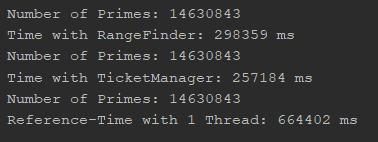
\includegraphics[scale=0.6]{Output_power_14.png} \\
			Because I ran the test before I have implemented the "terminating times" of each thread there are only the "full-terminating times".
			\subsubsection*{\textsc{RangeFinder}}
			\begin{adjustwidth}{1em}{}
				The \textsc{RangeFinder}-Threads takes 298359ms to finish searching for primes.
			\end{adjustwidth}
			\subsubsection*{\textsc{Ticketing-System}}
			\begin{adjustwidth}{1em}{}
				Now the \textsc{Ticketing-System} is significantly faster than the \textsc{RangeFinder} with only 257184ms.
			\end{adjustwidth}
			\subsubsection*{\textsc{One-Thread-Reference + Speedup}}
			\begin{adjustwidth}{1em}{}
				The \textsc{One-Thread-Reference} needs 664402ms, the speedup is therefore: \\
				\begin{enumerate}[]
					\item \textsc{RangeFinder-SpeedUp}: \\
					$\textit{SpeedUp} \ = \ \frac{\textit{OldExecutionTime}}{\textit{NewExecutionTime}} \ = \ \frac{664402}{298359} \ = \ 2.227$
					\item \textsc{Ticketing-System-SpeedUp}: \\
					$\textit{SpeedUp} \ = \ \frac{\textit{OldExecutionTime}}{\textit{NewExecutionTime}} \ = \ \frac{664402}{257184} \ = \ 2.583$
				\end{enumerate}
				\hfill \\
				In this case we can see that the \textsc{RangeFinder} is approximately 2 times faster than the sequencial approach. The \textsc{Ticketing-System} is even 2.5 times faster. This also adds to the previous case so we can say that these might be the general speedup-factors for the algorithms.
			\end{adjustwidth}
		\end{adjustwidth}
		
		\subsection*{Conclusion}
		In the end we can say that the \textsc{RangFinder} approach is approximately more than 2 times faster and the \textsc{Ticketing-System} approximately 2.5 times faster than the sequencial variant of the algorithm.
	\end{adjustwidth}	
\end{document}